% Created 2020-11-16 Mon 17:27
% Intended LaTeX compiler: pdflatex
\documentclass[11pt]{article}
\usepackage[utf8]{inputenc}
\usepackage[T1]{fontenc}
\usepackage{graphicx}
\usepackage{grffile}
\usepackage{longtable}
\usepackage{wrapfig}
\usepackage{rotating}
\usepackage[normalem]{ulem}
\usepackage{amsmath}
\usepackage{textcomp}
\usepackage{amssymb}
\usepackage{capt-of}
\usepackage{hyperref}
\usepackage{minted}
\IfFileExists{./resources/style.sty}{\usepackage{./resources/style}}{}
\IfFileExists{./resources/referencing.sty}{\usepackage{./resources/referencing}}{}
\addbibresource{./resources/references.bib}
\usepackage[mode=buildnew]{standalone}
\usepackage{tikz}
\usetikzlibrary{decorations.fractals}
\usetikzlibrary{lindenmayersystems}
\author{Ryan Greenup}
\date{\today}
\title{}
\hypersetup{
 pdfauthor={Ryan Greenup},
 pdftitle={},
 pdfkeywords={},
 pdfsubject={},
 pdfcreator={Emacs 27.1 (Org mode 9.4)}, 
 pdflang={English}}
\begin{document}

\tableofcontents


\section{Cauchy Integral Formula}
\label{cauchy-integral-formula}
This is from section 54 of the book, isn't it nice that it more or less
just works hey? \cite{zhangMakingEigenvectorBasedReputation2004}

\begin{align}
f\left( a \right) \frac{1}{2\pi i} \oint \frac{f\left( z \right)}{z- a}\mathrm{d}z
\end{align}

In view of this equation then: \cite{zhangMakingEigenvectorBasedReputation2004}

$$\begin{aligned}
\left| \int_C \frac{f\left( z \right)}{z- z_0} \mathrm{d}z - 2 \pi i f\left( z_0 \right) \right|<2 \pi \varepsilon
\end{aligned}$$

Some Images: \cite{ngStableAlgorithmsLink2001}

\begin{figure}[htbp]
\centering
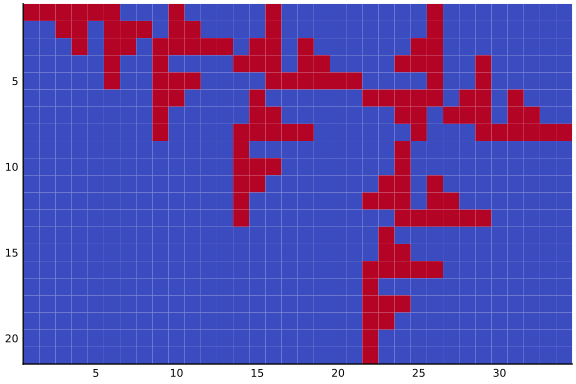
\includegraphics[width=12cm]{media/my-self-rep-frac.png}
\caption{\label{testim}This image is for testing purposes \cite{moskowitzLibraryGuidesWikipedia}}
\end{figure}

\begin{figure}[htbp]
\centering

\includegraphics[width=12cm]{media/tikz/Snowflake.png}
\caption{\label{testtikzins}This is a tikz image inserted as a png from imagemagick}
\end{figure}


\begin{figure}
\label{testtikzstd}
\caption{this is an example of embedded tikz lkasjdf lkjasdf }
\includestandalone[]{./media/tikz/Snowflake}
\end{figure}



\subsection{Heading 2}
\label{heading-2}
\subsubsection{Heading 3}
\label{heading-3}
\begin{minted}[]{sh}
  echo "Hello World"
\end{minted}


\paragraph{Heading 4}
\label{heading-4}
\subparagraph{Heading 5}
\label{heading-5}
\begin{enumerate}
\item Heading 6
\label{heading-6}
Arbitrary Code:

\begin{minted}[]{sh}
  n/bash

  # Print Help
  if [ "$1" == "-h" ]; then
      echo "Usage: `basename $0` <Format> <CSS>"
      style=~/Dropbox/profiles/Emacs/org-css/github-org.css
      exit 0
  fi

  # Make a working File from clipboard
  filename=lkjdskjjalkjkj392jlkj
  xclip -o -selection clipboard >> $filename
  LocalFile=$filename.org

  pandoc -s  -f org -t gfm $filename -o $filename

  echo "
  This was converted from `org` to `md` using `pandoc -t gfm` at time:
  $(date --utc +%FT%H-%M-%S)
  " >> $filename

  cat $filename | xclip -selection clipboard
  rm $filename

  nv & disown
  echo "Conversion from Org Successful, MD is in Clipboard"

  exit 0
\end{minted}
\end{enumerate}
\end{document}
